\documentclass[10pt]{article}

\usepackage{tmlr}
\usepackage{amsmath,amssymb}
\usepackage{booktabs}
\usepackage{graphicx}
\usepackage{xcolor}
\usepackage{url}
\usepackage{placeins}
\usepackage{xeCJK}
\setCJKmainfont[BoldFont=FandolSong-Bold.otf]{FandolSong-Regular.otf}
\setCJKmonofont{FandolHei-Regular.otf}
\graphicspath{{figs/}}

\newcommand{\delp}{DeLP}
\newcommand{\gain}{\Delta\ell}
\newcommand{\dbwt}{\Delta\mathrm{BWT}}

\title{One Degree of Freedom Moves the Frontier, the Other Four Do Not:\\
A Preregistered Factorization of an Active-Dendrite Repair,\\
Its Architecture-Bound Supply, and Five Failed Escapes}
\author{\name Anonymous Author \email anonymous@example.com \\ \addr Anonymous Institution}

\begin{document}

\maketitle

\begin{abstract}
A companion audit established that a one-parameter bias repair to an
active-dendrite continual learner acts as a structured-capacity intervention,
and conjectured that its gain--retention frontier could only be moved by
changing \emph{what} protection covers rather than \emph{when} it applies. We
test that conjecture and four adjacent escapes in a series of six
preregistered experiments (1{,}539 newly collected training runs plus $60$
reused controls, every criterion and Holm family
fixed before data collection, every deviation logged in an unmodified
preregistration). The five escapes of the title are the four failed
freedoms --- \emph{when}, $\lambda$, the forward intervention, and the
context pathway --- plus a fifth that fails loudest of all: the transfer
of the one freedom that works. \textbf{The conjecture holds on its home
architecture.}
Reallocating the anchor budget across past tasks under exact total-weight
conservation --- protecting recent tasks more, old tasks less --- moves the
frontier where two preregistered decay schedules and every scalar edit
failed: at $T{=}20$ it adds $\gain=+8.08$ over the un-repaired baseline while
\emph{improving} retention versus the repair itself
($\dbwt=+1.52$ vs.\ the repair, Holm $p=6.4\times10^{-5}$; four inherited
success criteria met in full), and the direction is specific --- protecting
\emph{old} tasks instead is worse on retention in all $20/20$
paired seeds. \textbf{But the supply of this degree of freedom is
architecture-bound, and we map its boundary three ways.} On a
calibrated real backbone (ResNet-18+GN, $\lambda$ re-calibrated to $0.1$) the
same reallocation does nothing ($n{=}20$: $\gain=+0.72$, $p=0.34$, seed
directions 11 positive / 9 negative) --- after a first round at $n{=}10$ had \emph{appeared} to
transfer ($+1.94$, Holm $p=0.041$), a preregistered extension clause exposed
the small-sample artifact, a flip we report in full. On the convolutional
toy backbone, sweeping $\lambda$ across four decades shows the companion
audit's ``repair collapses on conv'' was partly a single-$\lambda$ artifact
($\lambda{=}1000$: $+0.19$, n.s.; $\lambda\le316$: $+0.80$ to $+1.04$,
Holm-significant in $4/6$ points) yet the restored effect remains an order of
magnitude below its MLP value. A preregistered Transformer extension
completes the transfer map at a third trunk family: with both
architecture constants re-measured from scratch ($G$ frozen by probe,
$\lambda^{*}{=}100$ from a 120-run sweep), the reallocation is again
inert ($n{=}40$: $\gain=+0.09$, n.s.\ at a detectable threshold of
$\approx$0.2\,pp --- a measured zero, not a missed effect) while the gate
normalization itself transfers cleanly ($+7.01$, $40/40$ paired seeds
positive): the two freedoms the MLP conflates --- normalization and
direction --- separate across architectures. Finally, training-time corruption of the
task context itself --- pushed through forward pass, gradient mask, and
anchor statistics simultaneously --- leaves final accuracy untouched (24
Holm-corrected cells --- two consumption modes $\times$ three corruption
strengths $\times$ two dose levels $\times$ two datasets; minimum
$p=0.585$), extending a prior evaluation-time
null to training, and we show why this null admits a trivial competing
explanation (a constant gate that cannot carry information) that the audit's
three-instrument protocol can localize. We distill the process into eight
preregistration-gate failures we caught by fixed discipline rather than
post-hoc judgment, each documented with the diagnostic that distinguished
implementation error from clause conflict. The pattern across all six
experiments is a repair with exactly one live degree of freedom whose reach
is set by the trunk it sits on.
\end{abstract}

\section{Introduction}
\label{sec:intro}

Active-dendrite continual learners interleave two mechanisms: a dendritic
segment competition that routes each input, and usage-localized consolidation
(\delp{}) that protects past work by weighting per-neuron Fisher anchors with
segment usage. A companion audit \citep{zhou2026delp,zhou2026anchorbudget} established, across ten
preregistered findings, that the family's one-parameter bias repair is best
understood as a \emph{structured-capacity} intervention: its learning-term
gain is reproduced by scaling the protection strength $\lambda$ alone, its
retention cost concentrates on recent tasks, and changing \emph{when} the
intervention applies --- two preregistered decay schedules --- does nothing
to separate gain from forgetting. The audit ended with a conjecture, stated
as the natural next experiment: that the gain--retention frontier can only
be moved by changing \emph{what} the protection covers.

This paper is the systematic test of that conjecture and of every adjacent
escape we could preregister. It comprises six experiments, R1--R4 plus a
transfer extension R2T --- $1{,}539$ newly collected training runs and $60$
reused audit controls, across two datasets, five architectures, and a real
backbone. Every experiment was run under a written
preregistration whose success criteria, failure criteria, statistical
families, and conditional triggers were fixed before any data was collected;
where a gate failed or a clause had to be revised, the preregistration was
left unmodified and the deviation was recorded in a separate revision note.
Section~\ref{sec:discipline} summarizes this process because we believe it
is itself a contribution: eight implementation-gate failures, each caught by a
deterministic check rather than judgment, each with a different root cause.

\paragraph{The five questions.} Let $a_1,\dots,a_v$ be the Fisher anchors
accumulated after $v$ tasks, each with weight implicitly $1$. The repair
(retaining normalization of the gated trunk) sits on top of these anchors.
The degrees of freedom available to a practitioner are: (i) \emph{what} the
budget protects --- the per-anchor weights $w_j$; (ii) \emph{when} it applies
--- the audit's decay schedules, already falsified; (iii) \emph{how strongly}
--- $\lambda$, shown by the audit to be the dominant scalar axis; (iv) the
\emph{forward} intervention itself; and (v) the \emph{context pathway} that
supposedly routes tasks. We preregister one experiment per remaining
freedom and report all of them regardless of outcome.

\paragraph{Findings.}
\textbf{F1 (what):} budget direction is live on the home architecture ---
weight conservation notwithstanding, shifting weight toward recent tasks
under $\sum_j w_j = v$ moves the frontier (four inherited criteria, Holm
$p=6.4\times10^{-5}$), and the direction is causal ($20/20$ paired seeds
reverse when the weights point at old tasks). Specificity controls show the
effect requires the repaired forward pass: reallocation without it improves
retention but produces no gain, and raising $\lambda$ alone slides
\emph{along} the frontier rather than moving it.
\textbf{F2 (transfer):} the same intervention is inert on a calibrated
ResNet-18+GN backbone at $n{=}20$ --- and we report the $n{=}10$ round that
first appeared positive and was overturned by the preregistered extension,
as a concrete instance of a discipline preventing a false positive ---
and inert again on a Transformer at $n{=}40$ with both architecture
constants recalibrated from scratch, while the normalization itself
transfers there cleanly: the supply map gains a third point, and the two
freedoms separate.
\textbf{F3 ($\lambda$ attribution):} the companion audit's conv collapse was
partly a single-point artifact; sweeping $\lambda$ restores a significant but
order-of-magnitude-smaller effect, with the audit's chosen $\lambda$
sitting exactly at the collapse point.
\textbf{F4 (context):} training-time task-label corruption through all three
consumption sites leaves accuracy untouched, with a structural competing
explanation we make explicit rather than claim robustness.
\textbf{F5 (process):} eight gate failures, all caught by fixed checks; we
extract portable rules.

\paragraph{Contributions.}
(1)~A preregistered confirmation, with full specificity controls, that
anchor-budget \emph{direction} is the second live degree of freedom of this
repair family, and that it is the only one besides $\lambda$.
(2)~A four-architecture boundary map of where that freedom runs out: real
backbone (no effect at $n{=}20$), mis-calibrated toy conv (effect masked at
the audited $\lambda$, restored but $19\%$ strength elsewhere), Transformer
(no effect at $n{=}40$ with recalibration, while normalization transfers at
$40/40$ seeds), and the context pathway (structurally unable to carry the
signal).
(3)~A methods section documenting eight preregistration-gate failures and
their diagnoses, which we argue should accompany any paper claiming
preregistered discipline.
(4)~A fully scripted reproduction package (independent recomputation of
every headline number from raw run records, 25/25 checks passing on two
machines).

\section{Background and Setting}
\label{sec:setting}

We inherit the companion audit's protocol in full; we restate only what the
new experiments manipulate. The learner is the bare-MLP active-dendrite
network of the audit (width $256$, $n_{\mathrm{seg}}{=}T$, kWTA keep-rate
$25\%$, protected gradients on), trained on Permuted-MNIST and
Permuted-Fashion with $T\in\{10,20\}$ tasks, Adam, oracle task context at
evaluation. Metrics are the learning term $\ell$ (mean just-learned
accuracy), final average $\bar{a}$, and backward transfer
$\mathrm{BWT}$; all comparisons are paired by (dataset, seed) with
$n{=}10$ per dataset, $n{=}20$ pooled, two-tailed, Holm-corrected within
families fixed in the preregistrations.

\begin{table}[t]
\centering
\caption{Training protocol, inherited verbatim from the companion audit
per backbone. One row per hyperparameter; nothing in any column was tuned
by this paper. MLP and conv share the audit's full training stack
(optimiser, schedule, sample budget); ResNet-18+GN carries the audit's
external-validity calibration, in which the only re-calibrated quantity is
$\lambda$ (and the repair's $G$); the Transformer (R4) re-measures both
constants from scratch by preregistered probe and sweep.}
\label{tab:protocol}
\footnotesize
\setlength{\tabcolsep}{3pt}
\begin{tabular}{lllll}
\toprule
 & bare MLP (R1, R2) & toy conv (R3) & ResNet-18+GN (R2T) & Transformer (R4) \\
\midrule
datasets & Permuted-MNIST / & Permuted-MNIST / & Split-CIFAR-100 & Permuted-MNIST / \\
         & Permuted-Fashion & Permuted-Fashion & (task-IL) & Permuted-Fashion \\
tasks $T$ & $10,\,20$ & $10$ & $10$ & $20$ \\
trunk & MLP, width $256$ & 4-layer conv, & ResNet-18+GN, & 2-layer Transf., \\
      & one segment/task & bias-free, width $2048$ & pooled width $512$ & $d{=}256$, pooled $512$ \\
segment keep (kWTA) & $25\%$ ($64/256$) & $25\%$ & $25\%$ ($128/512$) & $25\%$ ($128/512$) \\
optimiser & Adam, $lr{=}10^{-3}$ & Adam, $lr{=}10^{-3}$ & SGD, $lr{=}5{\times}10^{-2}$ & Adam, $lr{=}10^{-3}$ \\
momentum / weight decay & -- & -- & $0.9$ / $5{\times}10^{-4}$ & -- \\
gradient clip & -- & -- & global norm $5.0$ & -- \\
batch / epochs per task & $256$ / $2$ & $256$ / $2$ & $128$ / $5$ & $256$ / $2$ \\
train samples per task & $10{,}000$ & $10{,}000$ & $5{,}000$ ($10$ classes) & $10{,}000$ \\
$\lambda$ (audited) & $1000$ & $1000$ & $0.1$ & $100$ (sweep) \\
gate constant $G$ & $0.565$ & $0.565$ & $0.5749$ & $0.5827$ (probe) \\
\bottomrule
\end{tabular}

\vspace{2pt}
\raggedright\footnotesize Task identity is seeded per seed (generator seed
$100{+}\text{seed}$): within a seed, every arm sees identical task
permutations (MLP/conv/Transformer) or identical class orders (ResNet),
which is what makes the paired comparisons exact. The conv trunk is
$32{\to}64{\to}128{\to}2048$ channels, $3{\times}3$, stride
$1/2/2/2$, no bias anywhere. $G$ is the measured constant gate
expectation, per backbone; the repair divides the trunk by it. The R4
column's $\lambda$ and $G$ are this paper's own calibration outputs
(Section~\ref{sec:r4}), not inherited values.
\end{table}

The repair under study deletes the sigmoid gate and rescales the trunk by
$1/G$ with $G$ the measured constant gate expectation
\citep{zhou2026delp,zhou2026anchorbudget}; we call this arm \texttt{renorm}. Its anchors are the
per-neuron Fisher anchors of \delp{}, accumulated one per completed task
with unit weight. The audit's four success criteria for any candidate
frontier-mover at $T{=}20$: $\gain\ge+4.0$ over the un-repaired baseline,
$\dbwt\ge-0.5$, improvement of $\dbwt\ge+1.11$ over \texttt{renorm} itself
with Holm $p<0.05$, and no degradation at $T{=}10$. These are inherited
verbatim; we add nothing.

\section{Related Work}
\label{sec:related}

\paragraph{Regularization-based continual learning.}
The parameter-protection literature splits into two families. The
regularization family
\citep{kirkpatrick2017,zenke2017,aljundi2018,chaudhry2018}
concentrates its effort on one question: how should \emph{per-parameter}
importance be estimated --- Fisher information, path-integral accumulation,
sensitivity to perturbation --- and imposed; the isolation family masks or
prunes task-specific parameter subsets \citep{serra2018,mallya2018}. In
both, the estimated protection is a
measurement; the research variable is the estimator or the mask. This paper
holds the
estimator fixed (the audit's per-neuron Fisher anchors, inherited verbatim)
and varies a question upstream of estimation that neither family's design
space
otherwise exposes: how a \emph{per-anchor, task-level} protection
budget is \emph{allocated} across past tasks, under exact total-weight
conservation that removes regularization mass as a confound. On that axis
the families' own knobs are scalar-, schedule-, or mask-shaped --- a global
$\lambda$
\citep{kirkpatrick2017}, online decay of consolidation strength
\citep{chaudhry2018}, hard attention masks \citep{serra2018} --- which is
precisely the \emph{strength/schedule} axis the companion audit found
exhausted and this paper's R3 re-quantifies. Context-dependent gating, the
mechanism whose repair created these anchors, has its own lineage
\citep{masse2018}; R1 tests whether its context pathway matters in training.
Surveys delimit the same axes \citep{delange2022,parisi2019}; to our
knowledge no prior continual-learning work isolates a direction-of-allocation
effect under exact budget conservation.

\paragraph{Dendritic computation.}
The structural substrate --- compartmentalized dendrites computing
context-dependent nonlinearity
\citep{poirazi2020,ujfalussy2018}, consolidation dynamics \citep{benna2016},
and dendritic gating of plasticity \citep{onasch2026} --- motivates treating
the anchor population as structured capacity rather than a scalar
regularizer; the companion audit's gate-constant finding and this paper's
direction specificity are the quantitative expression of that framing.

\paragraph{Methodology.}
The discipline apparatus follows the preregistration and honest-reporting
line \citep{lipton2019,musgrave2020,agarwal2021}: criteria and Holm families
fixed before data collection, sample-extension and reverse-trigger clauses
fixed in advance, every deviation logged against an unmodified
preregistration, and every number in this paper mechanically recomputed from
raw records.

\section{R2: The Anchor-Budget Direction}
\label{sec:r2}

\subsection{Intervention}
At phase $v$ with anchors $a_0,\dots,a_{v-1}$ of ages
$g_j = (v{-}1)-j$, replace the unit weights by
\begin{equation}
w_j \;=\; (1-\alpha) \;+\; \alpha\,\frac{v\,e^{-g_j/\tau}}{\sum_k e^{-g_k/\tau}},
\qquad \tau = T/4,
\label{eq:weights}
\end{equation}
so that $\sum_j w_j = v$ identically for every $\alpha$: total protection
strength is conserved phase by phase, and $\alpha{=}0$ reproduces the
audit's uniform penalty bit-for-bit (verified by an independent sentinel
grid, 40/40 pairs, maximum metric difference $0.0$). This conservation is
the design feature that isolates \emph{direction} from \emph{strength} ---
the audit had already shown $\lambda$ (strength) to be the dominant scalar
axis, and any ``direction'' result that quietly changed strength would be
uninterpretable. Nothing else changes: not the forward pass, not anchor
construction, not Fisher estimation, not evaluation.

\subsection{Preregistered criteria and arms}
The six arms are \texttt{base}, \texttt{renorm}, the candidates
\texttt{renorm\_rec05} ($\alpha{=}0.5$) and \texttt{renorm\_rec10}
($\alpha{=}1$), the specificity control \texttt{renorm\_lamup}
($\lambda{\times}3.13$ on \texttt{renorm}), and the interaction control
\texttt{base\_rec10} (reallocation without the repaired forward pass), over
$2$ datasets $\times\,T\in\{10,20\}\times10$ seeds ($240$ runs). The Holm
family is the two candidates' $\dbwt$ versus \texttt{renorm} at $T{=}20$,
fixed in advance.

\subsection{Result: the frontier moves}
\begin{table}[t]
\centering
\caption{R2 headline, pooled over datasets ($n{=}20$) with the per-dataset
decomposition of the two weakest quantities (learning-term difference
versus the repair; $n{=}10$ each). Criteria are evaluated on the pooled
statistics, inherited verbatim from the companion audit's closure grid;
the decomposition is reported, per the preregistration, because pooling
masks dataset asymmetry. Holm family = the two candidates' $\dbwt$
vs.\ \texttt{renorm} (pooled).}
\label{tab:r2}
\small
\setlength{\tabcolsep}{3.4pt}
\begin{tabular}{lcccccc|cc}
\toprule
 & \multicolumn{6}{c|}{pooled ($n{=}20$)} & \multicolumn{2}{c}{$\gain$ vs.\ \texttt{renorm}, split} \\
arm & $\gain$ & $\dbwt$ & $\dbwt$ vs.\ & $\gain$ & $\dbwt$ & Holm & MNIST & Fashion \\
 & ($T{=}20$) & ($T{=}20$) & \texttt{renorm} & ($T{=}10$) & ($T{=}10$) & $p$ & $T{=}20$ & $T{=}20$ \\
\midrule
\texttt{renorm\_rec05} & $+7.40$ & $-0.34$ & $+0.81$ & $+5.39$ & $+3.33$ & $1.4{\times}10^{-3}$ & $+0.10$ & $-0.58$ \\
\texttt{renorm\_rec10} & $\mathbf{+8.08}$ & $\mathbf{+0.37}$ & $\mathbf{+1.52}$ & $\mathbf{+5.84}$ & $\mathbf{+4.45}$ & $\mathbf{6.4{\times}10^{-5}}$ & $+1.10^{*}$ & $-0.22$ \\
\bottomrule
\end{tabular}

\vspace{2pt}
\raggedright\footnotesize Split columns: the learning-term difference
versus \texttt{renorm} within each dataset. $^{*}p{=}0.015$; the Fashion
split is negative ($-0.22$, $p{=}0.63$) --- on Fashion the reallocated
repair matches rather than exceeds the repair's learning term, and the
pooled $\dbwt$-versus-repair improvement is what carries the frontier
claim there. Both splits are secondary descriptions; all criteria are
pooled, as preregistered.
\end{table}
Table~\ref{tab:r2}: \texttt{renorm\_rec10} meets all four inherited
criteria; $\gain$ seed directions are $20/20$; we report honestly that
$\dbwt$-versus-\texttt{renorm} directions are $18/20$, short of the strict
unanimity form, and we do not downgrade the criterion to pass it. The
preregistered reverse-weighting trigger fired: protecting \emph{old} tasks
(\texttt{renorm\_anti10}) yields \emph{higher} learning
($\gain=+11.62$) but collapses retention ($\dbwt=-6.68$;
versus \texttt{rec10}: $-7.05$, $20/20$ paired seeds, $|d_z|=4.0$).
Direction, not strength or schedule, is the carrier.

\begin{figure}[t]
\centering
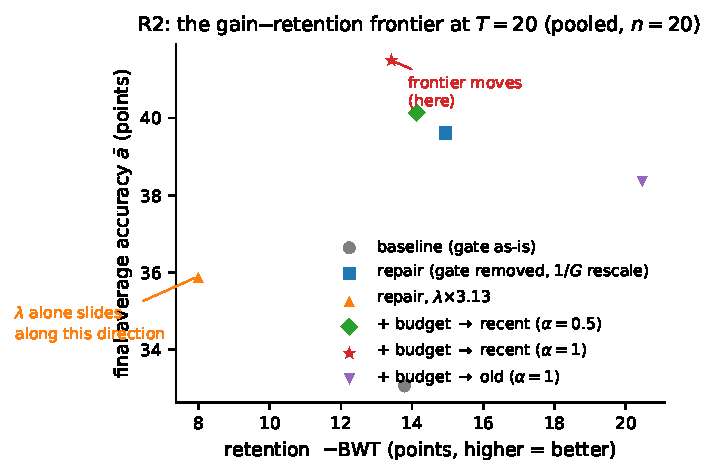
\includegraphics[width=0.62\linewidth]{figs/fig_frontier.pdf}
\caption{The $T{=}20$ gain--retention plane (pooled over both datasets,
$n{=}20$; horizontal axis is retention $-\mathrm{BWT}$, higher is better).
The recency-reallocated repair (\texttt{renorm\_rec10}, red star) sits
above and to the right of the repair itself: the frontier moves.
Raising $\lambda$ alone (orange triangle) moves along the
retention--accuracy trade-off, off the frontier. Redirecting the same
budget toward \emph{old} tasks (purple) recovers retention but pays
$3.2$ points of final accuracy: the direction of the budget, not its
existence, carries the effect.}
\label{fig:frontier}
\end{figure}

Figure~\ref{fig:frontier} places the six arms on the gain--retention
plane. Two readings matter. First, \texttt{renorm\_rec10} dominates
\texttt{renorm} in both coordinates --- this is what ``moving'' a frontier
means, as opposed to sliding along it, and the $\lambda$-only control
(\texttt{renorm\_lamup}) traces exactly such a slide. Second, the
reverse-weighting arm is \emph{not} a mirror image of the baseline: it
buys retention with learning, confirming that the budget is a real
instrument with a direction, not a scalar knob in disguise. The shape
hyperparameters ($\tau{=}T/4$, $\alpha\in\{0.5,1\}$) were fixed in the
preregistration and never scanned; the reverse-weighting arm uses the
identical shape with the sign flipped, so the $20/20$ reversal is itself
evidence that the finding is not an artifact of one favorable weighting
profile --- a shape-sensitive artifact would not survive its own mirror.

\subsection{Specificity: what the result is \emph{not}}
Two controls prevent two over-reads. \texttt{renorm\_lamup}
($\dbwt$ vs.\ \texttt{renorm} $=+6.94$, larger than the candidate's)
\emph{loses} $2.66$ points of learning: raising strength slides along the
frontier (retain more, learn less) --- it does not move it, and the
preregistered downgrade clause (``if strength-only also qualifies, the claim
collapses'') does not trigger. \texttt{base\_rec10} improves retention
($+2.25$) with \emph{no} gain ($-0.44$): reallocation alone is a retention
instrument; only on the repaired forward pass does it move the frontier.
The claim is therefore exactly: \emph{on the repaired baseline, budget
direction moves the frontier}; not ``recency weighting is a general
continual-learning improvement.''

\section{R2T: The Boundary on a Real Backbone}
\label{sec:r2t}

The companion audit's external-validity arm had already shown the repaired
forward pass itself is the \emph{worst} gate manipulation on ResNet-18+GN /
Split-CIFAR-100 ($-8.83$). R2T asks the orthogonal question: does
\emph{budget direction} survive where the forward intervention does not?
Protocol is the audit's, inherited verbatim by import ($\lambda{=}0.1$, its
per-architecture calibration; $G{=}0.5749$; SGD; task-IL; 10 seeds):
Split-CIFAR-100 as ten tasks of ten classes each, all $5{,}000$ training
images per task, and a class order seeded identically across arms so that
paired comparisons remain exact
(Table~\ref{tab:protocol}, right column). New arms are
\texttt{base\_rec10} (reallocation only), \texttt{renorm\_rec10}
(both), and \texttt{base\_anti10}, against the audit's existing
\texttt{base}/\texttt{renorm} runs reused as shared controls.

\paragraph{The flip.} The first round ($n{=}10$) supported transfer:
$\gain(\texttt{base\_rec10} - \texttt{base}) = +1.94$, Holm $p=0.041$,
apparently qualifying as ``reallocation improves the un-repaired backbone
too.'' Three of four primary raw $p$-values fell in the preregistered
$(0.01,0.1)$ extension band, firing the sample-extension clause. At
$n{=}20$ --- new arms plus control arms rerun for the new seeds with the
audit's own trainer --- the effect collapsed to $+0.72$ ($p=0.34$, seed
directions 11 positive / 9 negative); the repaired-contrast collapsed
likewise. The preregistered verdict had three levels --- T1
transfer, T2 partial rescue (within the repaired arm only), T3 fail ---
and reads \textbf{T3}: the contrast did not even reach the partial-rescue
level. We report the $n{=}10$ round, its trigger, and the flip in the
main text, not an appendix: a discipline that only surfaces its
confirmations is advertising, not method. A further reason to distrust
the first round operates before any statistics: the R2T pairing is
\emph{cross-run} --- new arms trained in this paper's sessions, control
arms in the audit's --- and a design probe run \emph{before} the
preregistration, as environment characterization rather than R2T data,
measured same-seed reruns of the audit's own baseline arm differing by up
to $6.8$ learning-term points under cuDNN nondeterminism. That probe is
the reason R2T's preregistration contains no bit-identity gates and
relies on paired statistics instead. A
single-round Holm $p{=}0.041$ is exactly the kind of margin that
run-level noise can manufacture; the extension clause was designed for
marginal significances, and here it doubly earned its keep.
Figure~\ref{fig:flip} shows the per-seed deltas behind the flip: the
first round's nine positive seeds were not a stable majority but a lucky
draw, and the ten added seeds split $2$ positive / $8$ negative. The large
residual contrast
($\texttt{base\_rec10} - \texttt{renorm} = +10.06$, $20/20$ seeds) is
carried almost entirely by the repaired forward pass being harmful on this
backbone --- an audit finding, not a new one. Direction specificity is also
absent here (reverse weighting is statistically indistinguishable),
distinguishing the real backbone from the MLP, where it was $20/20$.

\begin{figure}[t]
\centering
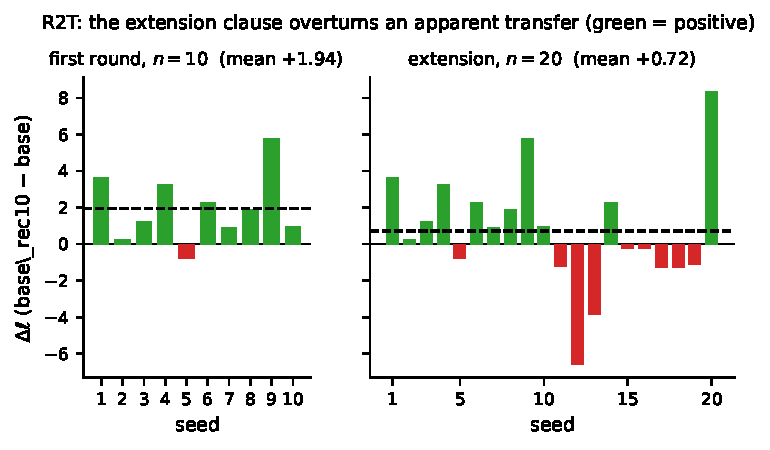
\includegraphics[width=0.78\linewidth]{figs/fig_flip.pdf}
\caption{R2T per-seed $\gain$ (reallocation minus baseline on
ResNet-18+GN). Left: the first round's $n{=}10$ seeds --- mean $+1.94$,
one strongly negative seed, enough for Holm-significance at $p=0.041$.
Right: the preregistered extension to $n{=}20$ --- the ten added seeds
split $2$ positive/$8$ negative, the mean collapses to $+0.72$
($p=0.34$), and the verdict flips from ``transfer'' to ``fail''.
Green bars are positive seeds.}
\label{fig:flip}
\end{figure}

\section{R3: The $\lambda$ Attribution on the Toy Conv}
\label{sec:r3}

The audit's threats-to-validity section conceded the conv collapse might be
a $\lambda$ mis-calibration artifact. R3 sweeps
$\lambda\in\{0,\,3.2,\,32,\,316,\,1000,\,3160\}$ on the audit's conv
backbone --- the audit's four-layer bias-free conv trunk on the same
Permuted-MNIST/Fashion tasks and the same training stack as the MLP
(Table~\ref{tab:protocol}), with the gate constant inherited unchanged
--- ($240$ runs; $\lambda{=}0$, never previously run, included; two arms
$\times$ two datasets $\times$ ten seeds per $\lambda$). The
preregistered two-sided criteria --- ``restoration'' ($\gain\ge+2$) versus
``boundary'' (all $|\gain|<1$, no trend) --- \emph{both} failed to fire:
the truth is in between, and more interesting than either. Learning-term
gain over the un-repaired arm is Holm-significant at $\lambda\le316$
($+0.80$ to $+1.04$, $4/6$ points) yet collapses exactly at the audit's
$\lambda{=}1000$ ($+0.19$, $p=0.57$), and the restored magnitude is
$19\%$ of the MLP value (the audit's $+5.48$ at the same $T$, same
protocol, same seeds). The curve has a second, shallower dip at
$\lambda{=}3160$ ($+0.64$, Holm $p=0.070$): the audit's single point sits
at the deepest of the two troughs. The audit's collapse was thus partly a
single-point artifact --- its one chosen $\lambda$ lands on the collapse
region of a non-monotonic dose curve, at its lowest point --- but
recalibration restores an
order-of-magnitude-smaller effect, not the repair. We state the correct
claim narrowly: single-$\lambda$ cross-architecture conclusions can
over- \emph{or} under-estimate; here it did both, in different directions
for significance and magnitude.

\begin{figure}[t]
\centering
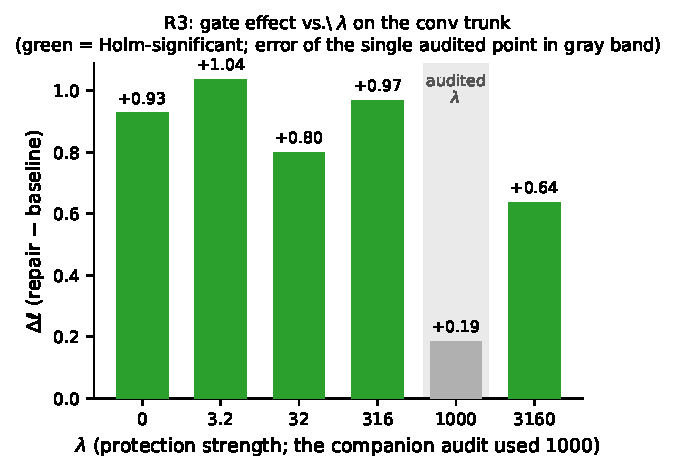
\includegraphics[width=0.6\linewidth]{figs/fig_lambda.pdf}
\caption{R3 dose curve: learning-term gain of the repair over the
un-repaired conv baseline, versus $\lambda$ (log axis; pooled $n{=}20$).
Green bars are Holm-significant. The companion audit's single audited
point ($\lambda{=}1000$, shaded) sits exactly at the collapse point of
the curve --- the one value at which the gate effect vanishes --- while
both weaker protection ($\lambda\le316$) and the $\lambda{=}0$ no-anchor
control show a significant but order-of-magnitude-smaller effect than
on the MLP ($+5.48$).}
\label{fig:lambda}
\end{figure}

\section{R1: The Context Pathway in Training}
\label{sec:r1}

An earlier evaluation-time probe had shown that corrupting the task context
at test time barely moves accuracy; the audit flagged training-time
corruption as the natural next experiment. R1 runs it: per-phase task
labels are mislabeled with probability $\rho\in\{0.1,0.2,0.4\}$
(a guaranteed-at-least-one sampling rule, after a preregistered gate caught
the Bernoulli version's mathematical conflict with a per-run positivity
clause), simultaneously through all three consumption sites --- forward
pass, gradient mask, and anchor Fisher/usage statistics --- against clean
controls and against a \emph{forward-only} arm (corruption at the
forward-pass site alone), whose contrast with the full corruption is the
preregistered anchor-chain test, $280$ authoritative runs. Nothing
transfers to accuracy: the
smallest Holm-corrected $p$ across all $24$ effect cells is $0.585$; the
preregistered anchor-chain hypothesis (corrupting anchor statistics costs
more than corrupting the forward pass alone) fails with
$|\Delta|\le0.42$; and the repair's bias gain survives corruption at
$93$--$112\%$ of its clean value. We explicitly refuse the robustness
reading: the audit's instruments show the gate constant ($0.564$ across
architectures) and the gradient-mask granularity inconsistent with the
forward read, so ``corrupting a pathway that structurally cannot carry
information'' is an equally sufficient explanation, and R1 cannot
distinguish the two. What R1 does establish, narrowly, is that
\emph{training-time label noise need not enter the acceptance checklist}
for this family on the audited trunks.

\section{R4: The Third Point on the Supply Map}
\label{sec:r4}

R2T left the supply boundary a two-point line: live on the bare MLP, dead
on a real convolutional trunk. A line cannot distinguish ``MLP-specific''
from ``everything except the MLP,'' so R4 adds a third point from a
different family: attention. A two-layer Transformer ($d_{\mathrm{model}}$
$256$, four heads, $28$ row-tokens mean-pooled into a $512$-d feature)
carries the same dendritic gate on its pooled features --- the audit's
attachment, with per-parameter Fisher anchors and the same $25\%$ kWTA
keep-rate --- on the same Permuted-MNIST/Fashion task stream at $T{=}20$,
with the R2 optimiser protocol inherited verbatim by import
(Table~\ref{tab:protocol}, right column). Nothing about the intervention
is rewritten: the recency weights are imported from the R2 module, and the
$\alpha{=}0$ identity is asserted constructively on the imported function
itself, not re-implemented.

\paragraph{Calibration.} Both architecture-relevant constants are
re-measured, not inherited. The gate constant is frozen from a base-arm
probe ($G=0.5827$, sd $0.0017$ over $120$ phase-probes; six runs), and
$\lambda$ is recalibrated by a preregistered $120$-run sweep over six
decades: the pooled reallocation-favorable gain (renorm $-$ base) rises
monotonically from $+2.71$ at $\lambda{=}0$ to $+7.10$ at
$\lambda^{*}{=}100$, then eases to $+7.00$ at $1000$ --- an inverted U
with no second trough, and no all-negative region, so the preregistered
fallback to the weaker contrast never fired. The main experiment ran at
the calibrated optimum with $n{=}40$ ($2$ datasets $\times\,20$ seeds,
paired by (dataset, seed); $200$ runs, five arms).

\paragraph{Result: T3 again --- and the map now has a trend.} All seven
implementation gates pass, including a calibration-consistency gate that
turns out to be bitwise: the Transformer driver is deterministic on this
stack, so scan and main runs agree to the last digit on the overlapping
seeds (the cuDNN nondeterminism that R2T measured at $6.8$ points on
ResNet does not occur here). The preregistered three-level verdict ---
inherited verbatim from R2T --- reads \textbf{T3}: reallocation is inert
within both bases (Table~\ref{tab:r4}: C1 $+0.07$, $p{=}0.33$; C2
$+0.09$, $p{=}0.14$; the Holm family of four is uniformly ns; seed
directions mixed at $+26/-14$ and $+26/-14$), and direction specificity is
absent for the second real-architecture time (anti vs.\ rec:
indistinguishable). The power note matters as much as the verdict: the
achieved paired sd is $0.37$--$0.45$ learning-term points, roughly an
order of magnitude below the conservative sd$=3$ the design assumed,
putting the detectable threshold at $\approx 0.2$\,pp --- the R2 effect
($+8.08$) would have registered at tens of standard deviations. This is a
measured zero, not a missed effect.

\begin{table}[t]
\centering
\caption{R4 headline on the Transformer ($T{=}20$, pooled over datasets,
$n{=}40$ paired by (dataset, seed)). C1/C2 enter the preregistered Holm
family (four tests); C3/C4 are exploratory descriptions, as in R2T. Arm
means ($n{=}40$ each): \texttt{base} $\ell=54.68$ / $\bar{a}=24.00$ /
$\mathrm{BWT}=-32.29$; \texttt{renorm} $61.69$/$23.99$/$-39.69$;
\texttt{base\_rec10} $54.75$/$23.77$/$-32.60$;
\texttt{renorm\_rec10} $61.77$/$24.05$/$-39.71$;
\texttt{base\_anti10} $54.68$/$23.79$/$-32.51$.}
\label{tab:r4}
\small
\setlength{\tabcolsep}{4pt}
\begin{tabular}{llcccc}
\toprule
 & comparison & $\gain$ & $\dbwt$ & $\gain$ split & Holm \\
 & & & & (MNIST / Fashion) & family \\
\midrule
C1 & \texttt{base\_rec10} $-$ \texttt{base}
   & $+0.07$ & $-0.31$ & $-0.06$ / $+0.20$ & ns \\
C2 & \texttt{renorm\_rec10} $-$ \texttt{renorm}
   & $+0.09$ & $-0.03$ & $+0.08$ / $+0.09$ & ns \\
C3$^{\dagger}$ & \texttt{base\_anti10} $-$ \texttt{base\_rec10}
   & $-0.07$ & $+0.09$ & --- & --- \\
C4$^{\dagger}$ & \texttt{base\_rec10} $-$ \texttt{renorm}
   & $-6.94$ & $+7.08$ & $0/40$ seeds & --- \\
\bottomrule
\end{tabular}

\vspace{2pt}
\raggedright\footnotesize $^{\dagger}$Exploratory, outside the family.
Holm family raw $p$: C1 $\ell$ $0.332$, C1 BWT $0.187$, C2 $\ell$
$0.145$, C2 BWT $0.904$; all Holm-adjusted $\ge 0.58$. C4:
$p=1.1\times10^{-24}$ ($\ell$), $4.4\times10^{-16}$ (BWT), and the
$\ell$ seed direction is $0/40$ --- the normalization effect is perfectly
sign-consistent even where its nominal carrier (reallocation) is inert.
Family $|d_z|$: $0.155$, $0.213$, $0.235$, $0.019$. C3 seed directions
are mixed in every metric --- direction specificity is absent on this
trunk.
\end{table}

\paragraph{What R4 adds: the two freedoms separate.} The negative verdict
is the least interesting thing in Table~\ref{tab:r4}. The gate
normalization itself --- the repaired forward pass, which the audit found
\emph{harmful} on ResNet ($-8.83$) --- transfers to attention cleanly:
renorm $-$ base $=+7.01$ with all $40/40$ paired seeds positive, and the
reverse contrast C4 pays back $-6.94$ with $0/40$ sign disagreements.
The supply claim therefore splits in two. The \emph{normalization}
freedom generalizes across all three tested trunks (MLP $+5.48$, conv
restored to $19\%$ strength by recalibration, Transformer $+7.01$); the
\emph{direction} freedom does not leave the MLP. ``Architecture-bound
supply'' stops being a binary line and becomes a three-architecture
trend, and the R2 claim inherits a sharper form: on the MLP, budget
direction and normalization were conflated in a single repaired forward
pass; the Transformer, where normalization works and direction does
nothing, shows they are mechanically independent.

\section{The Discipline: Eight Gate Failures}
\label{sec:discipline}

Every experiment above ran under a preregistration with
implementation-correctness gates whose failure voids the data. Eight times
a gate fired; none was resolved by relaxing a criterion.
Table~\ref{tab:gates} lists them with the diagnosis each demanded --- no
two share a root cause --- because the set illustrates what fixed checks
buy that judgment does not.

\begin{table}[t]
\centering
\caption{The eight implementation-gate failures. ``Resolution'' is what was
done to the \emph{data or code}, never to a criterion; every preregistration
file itself remained byte-identical throughout. Gates are deterministic
checks in the reproduction package, so each failure is replayable.}
\label{tab:gates}
\footnotesize
\setlength{\tabcolsep}{3.5pt}
\begin{tabular}{@{}llp{3.6cm}p{4.6cm}@{}}
\toprule
\# & exp. & gate that fired & root cause $\to$ resolution \\
\midrule
1 & R1 & positivity clause mathematically unsatisfiable &
prereg also specified Bernoulli sampling, but
$P(\text{zero mislabels}){=}(1-\rho)^T\!\neq\!0$ conflicts with a
per-run positivity requirement $\to$ resample with a
guaranteed-miss rule; all $280$ runs rerun (untouched runs verified
bit-identical) \\
2 & R2 & historical alignment &
reference data produced in a CPU era compared against GPU runs through a
discrete top-$k$ operator $\to$ regenerate references on the same device;
threshold unchanged \\
3 & R2 & equivalence evidence void &
the $\alpha{=}0$ equivalence proof lived in the pilot that gate~2 voided
$\to$ independent $80$-run sentinel grid, $40/40$ pairs bit-identical \\
4 & R2T & completeness check &
checker read a schema-incompatible field name
(\texttt{avg} vs.\ \texttt{final\_avg}) $\to$ fix the checker; data
untouched; zero analyses had leaked \\
5 & R3 & pilot crash &
conv anchor constructor had never executed on GPU (all historical conv
runs were CPU), exposing a latent device bug $\to$ runtime patch in the
sweep script only; upstream files unmodified \\
6 & R2T & sample-extension trigger &
fired on schedule at $n{=}10$ and \emph{overturned} the round's positive
conclusion $\to$ no resolution needed: the system working as designed \\
7 & R4 & weight conservation at $\lambda{=}0$ &
weights were computed from the anchor count, but a $\lambda{=}0$ run
builds no anchors --- empty weight vector fails conservation on the
first probe run $\to$ weights recomputed as a function of the phase
index (bit-identical for every $\lambda>0$); FAIL log retained \\
8 & R4 & checker pathway mismatch &
prereg required EPOCHS/BS/NTRAIN ``written and logged''; the driver
inherits them by import (the anti-drift device itself), so the checker's
source-text regex matched nothing and aborted before any statistics
$\to$ checker asserts the imported module constants; criterion values
unchanged \\
\bottomrule
\end{tabular}
\end{table}

The portable rules are stated in the reproduction package; we believe items
(1), (2), (7) and (8) in particular generalize to any preregistered
continual-learning program. A ninth, milder failure occurred at the
writing stage and is worth recording in the same spirit: an early draft
of Figure~\ref{fig:flip}'s caption described the added seeds as ``$3$
positive / $7$ negative'' and the first round as ``eight positive
seeds'' --- both written from the round means rather than counted from
the per-seed records (the true values are $2/8$ and nine). A scripted
check of every count and statistic against the raw run records caught
both; the rule we extract is that \emph{caption-level numbers deserve
the same programmatic verification as headline statistics}, because they
are quoted exactly as often and checked far less.

\section{Limitations}
\label{sec:limits}

All claims are bounded by the audited trunks (bare MLP, GN-MLP, 4-layer
conv, ResNet-18+GN, and R4's two-layer Transformer with the gate on its
pooled features), two permuted datasets and one split dataset,
$T\le20$, single insertion point for the gate, $n\le20$ per cell
(R4's pooled cells reach $n{=}40$). Larger Transformers, and Transformers
with explicit routing modules, remain untested (the audit's pin sentinel
would be the cheap first probe). The R2T flip means our transfer
claim is an $n{=}20$ null, not a mechanistic impossibility proof; cuDNN
nondeterminism on convolution bounds achievable reproducibility (measured:
same-seed reruns differ by up to $6.8$ learning-term points on ResNet),
which is why R2T's gates contain no bit-identity clauses --- while R4's
Transformer driver proved fully deterministic on its stack, letting its
calibration-consistency gate run bitwise. R3's dose curve
is six points on a log axis; we did not densify because the preregistered
densification trigger (restoration) did not fire, and R4's $\lambda$
sweep is likewise six decades at one depth. DeLP itself remains
non-competitive with replay baselines \citep{zhou2026delp,zhou2026anchorbudget}; nothing here
changes that, and our subject is the structure of the repair's degrees of
freedom, not its leaderboard position.

\section{Conclusion}

One degree of freedom --- anchor-budget direction --- moves the
gain--retention frontier of an active-dendrite repair on the trunk where
its supply exists, with clean direction specificity and specificity
controls. Four other escapes fail in instructing ways: recalibration
restores a shadow of the effect on the toy conv and nothing on the real
backbone or the Transformer --- where, however, the normalization itself
transfers at $40/40$ seeds, showing the two freedoms the MLP conflates
are mechanically independent; the context pathway cannot carry the
signal in training any more than at evaluation; and the discipline that
produced these answers caught eight implementation failures, one of
which overturned a positive result we would otherwise have reported.
The repair family is now mapped across five trunks: its reach
is set by the trunk it sits on, and the map is the contribution.

\subsubsection*{Reproducibility}
All experiments are scriptable from the reproduction package
(\texttt{r\_repro/}): preregistrations, revision notes, raw run records,
and an independent verifier that recomputes every headline number in this
paper from raw JSON (\texttt{python r\_repro/verify\_package.py}, 25/25
checks; verified on two machines). The $1{,}539$ newly collected runs
decompose as $1{,}506$ authoritative --- R1 grid $280$ plus its dose
probe $140$; R2 grid $240$, $\alpha{=}0$ sentinel $80$, GPU-reference
$80$, anti arm $40$; R2T $30{+}30{+}20$; R3 grid $240$; R4 gate probe
$6$, $\lambda$-sweep $120$, main grid $200$ --- plus $33$
pilot runs; the $280$ runs of R1's voided first grid are excluded from
every count. A second, paper-level checker
(\texttt{python check\_paper\_numbers.py}, 27/27 checks) re-derives the
seed-direction counts, per-dataset splits, figure-caption numbers, and
every protocol-table constant from
the same raw JSON and asserts their agreement with the text --- including
a regression rule raised from this project's ninth gate failure:
caption-level numbers are verified by script, not by eye. R4 contributes
its driver, calibration-sweep and main-grid JSONs, its analyzer, and its
preregistration/revision/report documents under \texttt{results\_r4/}.
Gate
arithmetic, Holm families, and trigger clauses are as fixed in the
preregistrations; deviations are logged, preregistrations unmodified.

\bibliographystyle{tmlr}
\bibliography{refs}

\end{document}
